\documentclass{article}\usepackage[]{graphicx}\usepackage[]{color}
%% maxwidth is the original width if it is less than linewidth
%% otherwise use linewidth (to make sure the graphics do not exceed the margin)
\makeatletter
\def\maxwidth{ %
  \ifdim\Gin@nat@width>\linewidth
    \linewidth
  \else
    \Gin@nat@width
  \fi
}
\makeatother

\definecolor{fgcolor}{rgb}{0.345, 0.345, 0.345}
\newcommand{\hlnum}[1]{\textcolor[rgb]{0.686,0.059,0.569}{#1}}%
\newcommand{\hlstr}[1]{\textcolor[rgb]{0.192,0.494,0.8}{#1}}%
\newcommand{\hlcom}[1]{\textcolor[rgb]{0.678,0.584,0.686}{\textit{#1}}}%
\newcommand{\hlopt}[1]{\textcolor[rgb]{0,0,0}{#1}}%
\newcommand{\hlstd}[1]{\textcolor[rgb]{0.345,0.345,0.345}{#1}}%
\newcommand{\hlkwa}[1]{\textcolor[rgb]{0.161,0.373,0.58}{\textbf{#1}}}%
\newcommand{\hlkwb}[1]{\textcolor[rgb]{0.69,0.353,0.396}{#1}}%
\newcommand{\hlkwc}[1]{\textcolor[rgb]{0.333,0.667,0.333}{#1}}%
\newcommand{\hlkwd}[1]{\textcolor[rgb]{0.737,0.353,0.396}{\textbf{#1}}}%

\usepackage{framed}
\makeatletter
\newenvironment{kframe}{%
 \def\at@end@of@kframe{}%
 \ifinner\ifhmode%
  \def\at@end@of@kframe{\end{minipage}}%
  \begin{minipage}{\columnwidth}%
 \fi\fi%
 \def\FrameCommand##1{\hskip\@totalleftmargin \hskip-\fboxsep
 \colorbox{shadecolor}{##1}\hskip-\fboxsep
     % There is no \\@totalrightmargin, so:
     \hskip-\linewidth \hskip-\@totalleftmargin \hskip\columnwidth}%
 \MakeFramed {\advance\hsize-\width
   \@totalleftmargin\z@ \linewidth\hsize
   \@setminipage}}%
 {\par\unskip\endMakeFramed%
 \at@end@of@kframe}
\makeatother

\definecolor{shadecolor}{rgb}{.97, .97, .97}
\definecolor{messagecolor}{rgb}{0, 0, 0}
\definecolor{warningcolor}{rgb}{1, 0, 1}
\definecolor{errorcolor}{rgb}{1, 0, 0}
\newenvironment{knitrout}{}{} % an empty environment to be redefined in TeX

\usepackage{alltt}

\usepackage[T1]{fontenc}
\usepackage{hyperref}
\usepackage{longtable}
\usepackage{booktabs}
\usepackage{pdfpages}
\usepackage{lineno}

\hypersetup{
    colorlinks=true,       % false: boxed links; true: colored links
    urlcolor=blue           % color of external links
}

% Comments begin with a percent.
% define the title
\author{Brian J. Knaus, Javier F. Tabima and Niklaus J. Gr\"{u}nwald}
\title{Mitochondrial molecular markers for US lineages of \emph{P. infestans}}

% Begin the document.
\IfFileExists{upquote.sty}{\usepackage{upquote}}{}
\begin{document}
%\SweaveOpts{concordance=TRUE}

% generates the title
\maketitle
\newpage

% Abstract
%\begin{abstract}
%Morphometric analysis of \emph{Carex minicaulis}.
%\vspace{8pt}
%Keywords: \emph{Carex}; Morphometrics; Taxonomy.
%\end{abstract}
%\pagebreak

% insert the table of contents
\tableofcontents
\listoffigures
\listoftables

\newpage

%\newpage

%% ---------- ---------- ---------- Section ---------- ---------- ---------- %%

\linenumbers

\section{Samples}

The sample includes data which was opportunistically gathered from previous publications as well as data which is not yet available to the public (Judelson, unpublished).

\vspace{12pt}

\begin{center}
\begin{tabular}{ l c c }
  \hline
  Sample & Count & Reference \\
  \hline
  T30-4 & 1 & \cite{haas2009genome} \\
  PIC99189 \& 90128 & 2 & \cite{raffaele2010analyses} \\
  13\_a2 & 1 & \cite{cooke2012genome} \\
  Yoshida et al. & 13 & \cite{yoshida2013correction} \\
  Martin et al. & 3 & \cite{martin2013reconstructing} \\
  Judelson & 8 & NA \\
  \hline
  Total & 28 & \\
  \hline
\end{tabular}
\end{center}

\vspace{12pt}

\begin{itemize}

\item The sample `T30-4' was the first sequenced genome and is considered the reference for nuclear work \cite{haas2009genome}.  This genome was assembled prior to high-throughput sequencing (i.e., Illumina and 454 technologies).  The data presented here are not the sequences used for the paper but are part of a project by \href{http://www.broadinstitute.org/annotation/genome/phytophthora_infestans/MultiHome.html}{The Broad} to resequence this sample using Illumina and 454 technologies.

\item Note that both the Yoshida and Martin papers included ancient DNA in their analyses \cite{yoshida2013correction, martin2013reconstructing}.  Here we have omitted those samples and focused on modern samples.

\item For enigmatic reasons, not all of the samples from the Yoshida and Martin papers were actually available online.  Therefore our numbers here do not match those presented in the papers.  

\item The Judelson data include a sample of US1 which was sampled at three different time points (us1\_1, us1\_2 and us1\_3).  We suspect that these were different samples and not necessarily the same clone.  Therefore differences among these samples may either be due to biological or technical factors.

\item The Judelson data includes a sample of US8 which has been characterized as having fungicide resistance \cite{danies2013phenotypic}.  This lineage was also sequenced by Martin et al. \cite{martin2013reconstructing}.  These are most likely different samples so differences among these samples may be interpreted as biological.  
  
\item The Yoshida data includes one sample of \emph{P. mirabilis} (p7722), this should jump out in the analyses.

\item For the mitochondrial data we used the type IIa form \cite{avila2006mitochondrial} because it was the longest sequence and we felt this would provide the best alignment.

\end{itemize}

We've used the term `SNP' fairly loosely in this document.  The term `variant' may be more appropriate.  Until fairly recently the software tools we've been using could only handle SNPs.  They now report short indels as well.

%% ---------- ---------- ---------- Section ---------- ---------- ---------- %%

\section{Read mapping}

Reads were mapped to the type IIa mitochondrial reference \href{http://www.ncbi.nlm.nih.gov/nuccore/AY898627.1}{"AY898627.1"}.  Reads were mapped using bowtie2 \cite{langmead2012fast}.  Variants were called using SAMtools\cite{li2009sequence}.

\subsection{Variant filtering}
To check which of the calls are good calls, the variant files were filtered by quality, read depth and mapping quality (Figures \ref{fig:plot_unfilter},\ref{fig:plot_filter}). For this we used an in-house R package called \href{https://github.com/knausb/vcfR}{vcfR}. Sequencing depth is cumulative over all sampels.  Quality here is for each variant over all samples and ranges from 1-999.

The genotype caller in Samtools assumes a diploid, bi-allelic model.  Because mitochondrial are assumed to be haploid we tried to filter out heterozygous calls.  Samples which included high quality heterozygote calls (p1362, p6096, p10650, p12204, p10127) were mostly from the Yoshida et al. \cite{yoshida2013correction} paper and were among the low sequencing depth samples they included.  Because these samples are not among the US lineages we're interested in, and because they are apparently of low sequencing depth, we omitted them for now.  However, the sample nl07434 was among the high sequencing depth samples from this paper and is perhaps noteworthy.  T30-4 was called as a heterozygote for one variant and is perplexinng.

The variants remaining after filtering were visualized as a linear chromosome in Figure \ref{fig:chromogc}.





\begin{knitrout}
\definecolor{shadecolor}{rgb}{0.969, 0.969, 0.969}\color{fgcolor}\begin{figure}[p]

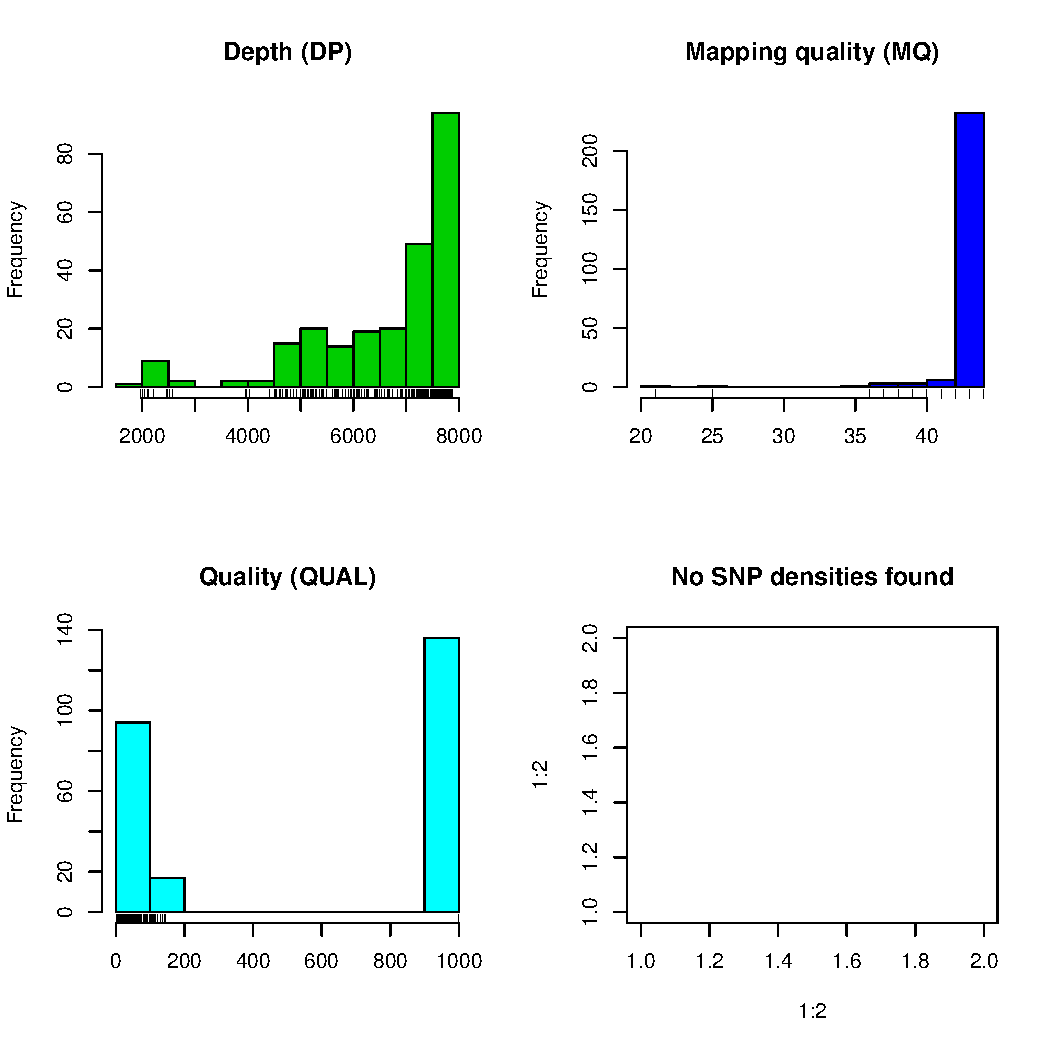
\includegraphics[width=\maxwidth]{figure/plot_unfilter} \caption[Quality results for the mtDNA SNP calls before filtering]{Quality results for the mtDNA SNP calls before filtering.\label{fig:plot_unfilter}}
\end{figure}


\end{knitrout}





\begin{knitrout}
\definecolor{shadecolor}{rgb}{0.969, 0.969, 0.969}\color{fgcolor}\begin{figure}[p]

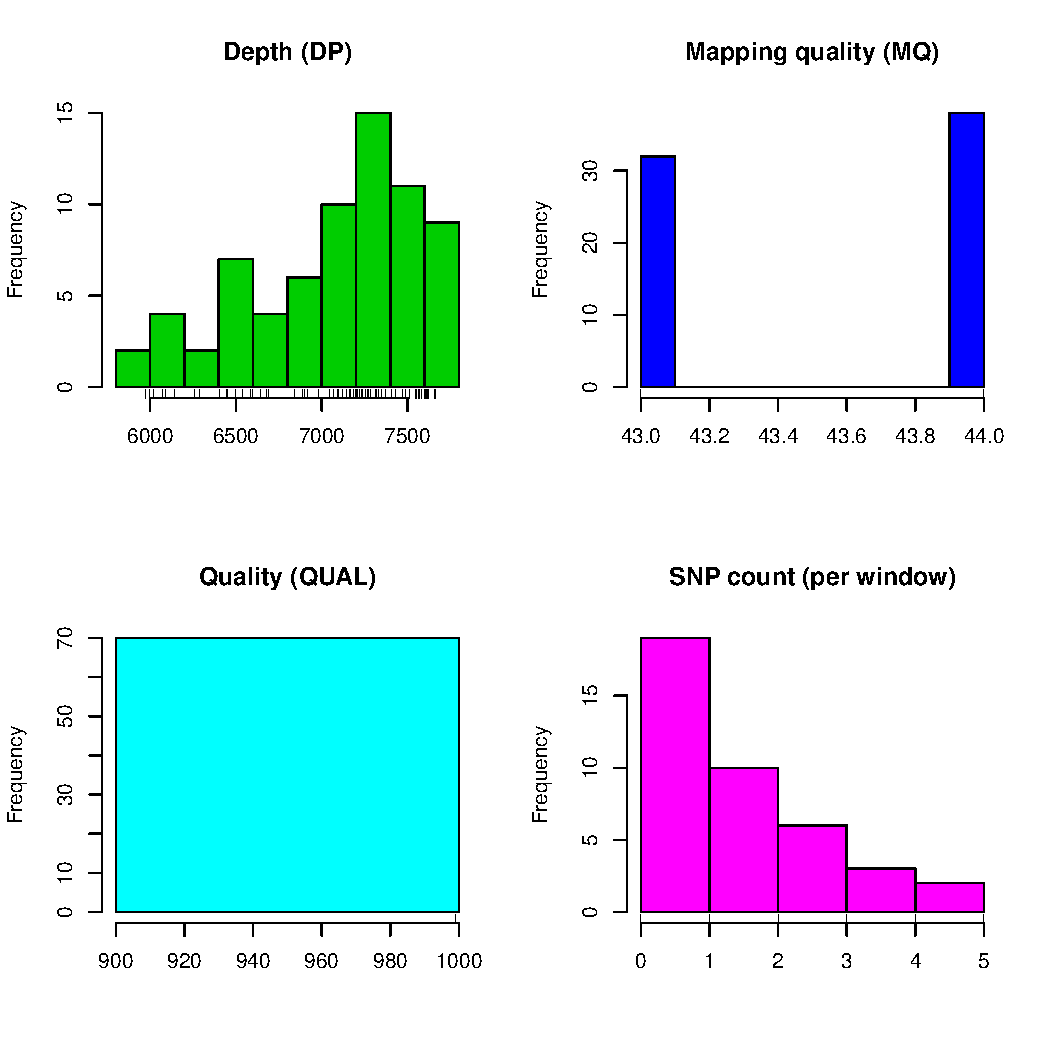
\includegraphics[width=\maxwidth]{figure/plot_filter} \caption[Quality results for the mtDNA SNP calls after filtering and windowizing variants]{Quality results for the mtDNA SNP calls after filtering and windowizing variants.\label{fig:plot_filter}}
\end{figure}


\end{knitrout}


\begin{knitrout}
\definecolor{shadecolor}{rgb}{0.969, 0.969, 0.969}\color{fgcolor}\begin{kframe}
\begin{verbatim}
## Before filtering:
## [1] 247
## After filtering:
## [1] 70
## gt.m2sfs is commented out
\end{verbatim}
\end{kframe}
\end{knitrout}


% latex table generated in R 3.0.2 by xtable 1.7-1 package
% Wed Feb 19 13:13:15 2014
\begin{table}[ht]
\centering
\begin{tabular}{llcccc}
  \hline
 & CHROM & POS & REF & ALT & Tree character \\ 
  \hline
6 & Supercontig\_1.1 & 2701 & C & T &   1 \\ 
  7 & Supercontig\_1.1 & 2728 & C & A &   2 \\ 
  12 & Supercontig\_1.1 & 3519 & G & T &   3 \\ 
  36 & Supercontig\_1.1 & 6872 & accc & acc &   4 \\ 
  42 & Supercontig\_1.1 & 7857 & A & G &   5 \\ 
  44 & Supercontig\_1.1 & 8118 & T & G &   6 \\ 
  59 & Supercontig\_1.1 & 9857 & T & C &   7 \\ 
  62 & Supercontig\_1.1 & 10146 & A & G &   8 \\ 
  85 & Supercontig\_1.1 & 13684 & A & G &   9 \\ 
  106 & Supercontig\_1.1 & 15563 & G & A &  10 \\ 
  114 & Supercontig\_1.1 & 16986 & G & A &  11 \\ 
  119 & Supercontig\_1.1 & 18440 & A & T &  12 \\ 
  123 & Supercontig\_1.1 & 19793 & G & A &  13 \\ 
  124 & Supercontig\_1.1 & 20005 & C & A &  14 \\ 
  125 & Supercontig\_1.1 & 20290 & G & T &  15 \\ 
  128 & Supercontig\_1.1 & 20464 & T & C &  16 \\ 
  141 & Supercontig\_1.1 & 22711 & G & A &  17 \\ 
  147 & Supercontig\_1.1 & 23431 & G & A &  18 \\ 
  150 & Supercontig\_1.1 & 23872 & G & T &  19 \\ 
  154 & Supercontig\_1.1 & 24611 & C & T &  20 \\ 
  159 & Supercontig\_1.1 & 25142 & A & C &  21 \\ 
  160 & Supercontig\_1.1 & 25204 & T & C &  22 \\ 
  161 & Supercontig\_1.1 & 25237 & G & T &  23 \\ 
  169 & Supercontig\_1.1 & 26684 & A & G &  24 \\ 
  171 & Supercontig\_1.1 & 26767 & T & C &  25 \\ 
  186 & Supercontig\_1.1 & 28680 & C & A &  26 \\ 
  187 & Supercontig\_1.1 & 28783 & A & G &  27 \\ 
  192 & Supercontig\_1.1 & 30427 & T & G &  28 \\ 
  193 & Supercontig\_1.1 & 30552 & A & G &  29 \\ 
  194 & Supercontig\_1.1 & 30591 & A & G &  30 \\ 
  195 & Supercontig\_1.1 & 30660 & C & T &  31 \\ 
  201 & Supercontig\_1.1 & 31403 & T & C &  32 \\ 
  221 & Supercontig\_1.1 & 35296 & G & T &  33 \\ 
  222 & Supercontig\_1.1 & 35367 & taaaaaaaaaaa & taaaaaaaaaa &  34 \\ 
  233 & Supercontig\_1.1 & 36663 & T & C &  35 \\ 
  239 & Supercontig\_1.1 & 37562 & C & T &  36 \\ 
  242 & Supercontig\_1.1 & 38345 & C & A &  37 \\ 
   \hline
\end{tabular}
\caption{Variants remaining after filtering.} 
\label{ptab}
\end{table}




\begin{knitrout}
\definecolor{shadecolor}{rgb}{0.969, 0.969, 0.969}\color{fgcolor}\begin{figure}[p]

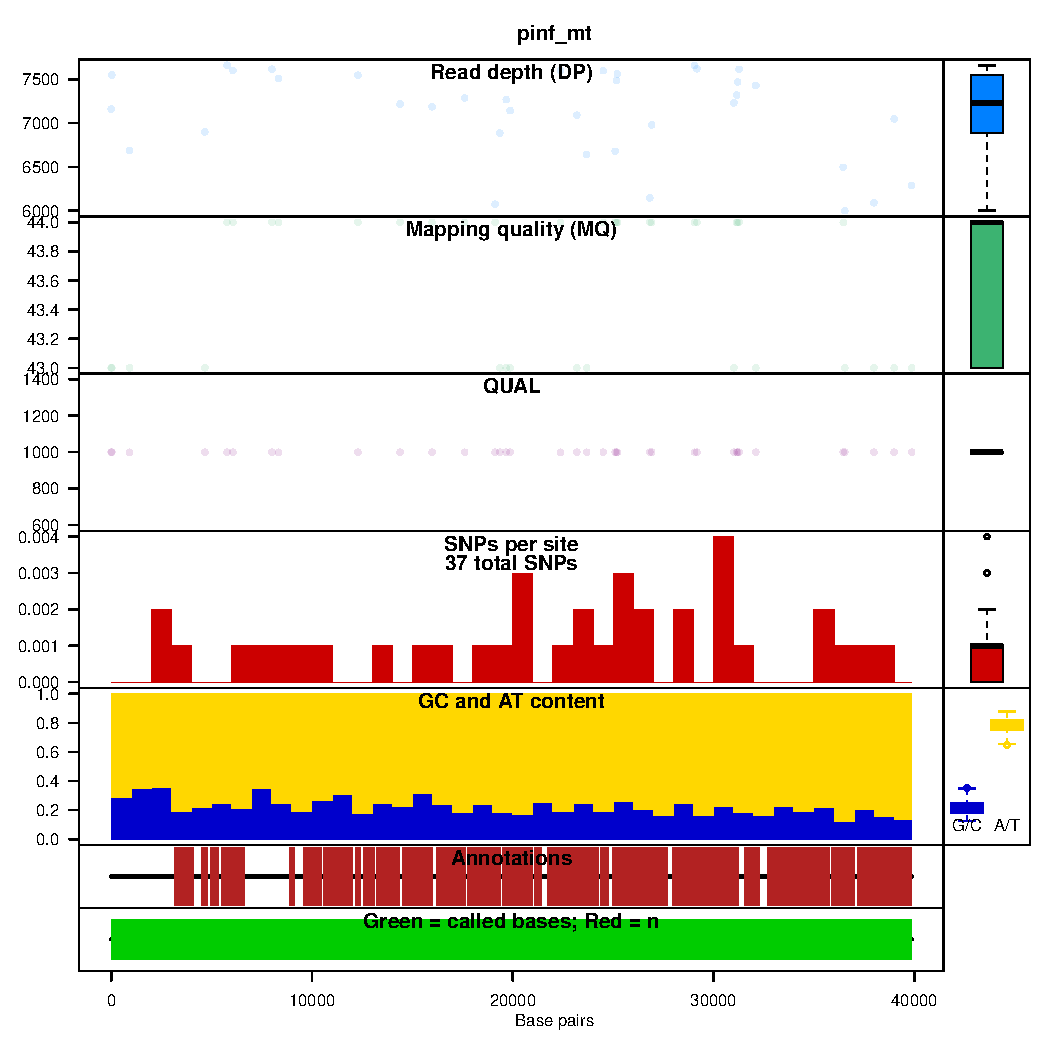
\includegraphics[width=\maxwidth]{figure/chromogc} \caption[Whole mtDNA genome scan for the P]{Whole mtDNA genome scan for the P. infestans samples.\label{fig:chromogc}}
\end{figure}


\end{knitrout}



%\section{SNPs after filtering}

Filtering the variant panel based on quality (QUAL=999), cumulative sequencing depth (1st quartile >= DP >= 3rd quartile) and mapping quality (1st quartile >= MQ >= 3rd quartile) resulted in 37 variants (Table \ref{ptab}).  We have identified a fraction of these as being diagnostic for a small group of samples (Table \ref{table:DiagSNP}).

%After filtering we proceeded to look at which of the SNP's were supported after the filtering (Table \ref{table:DiagSNP}).

\begin{table}[h!]
\centering
\caption{Diagnostic SNP positions for the mtDNA genome after filtering.}
\begin{tabular}{@{}lll@{}}
\toprule
Position & SNP & Diagnostic for       \\ \midrule
7857     & A/G & p10127, us11 and us1 \\
8118     & T/G & us1                  \\
20464    & T/C & p17777, us22 and us8 \\
22711    & G/A & p17777, us22 and us8 \\
26767    & A/G & p10127, us11 and us1 \\
28783    & A/G & p10127, us11 and us1 \\
36663    & T/C & us8                  \\ \bottomrule
\end{tabular}
\label{table:DiagSNP}
\end{table}

%% ---------- ---------- ---------- Section ---------- ---------- ---------- %%

\section{Variant segregation}
%\section{Diagnostic SNP mapping}

In order to visualize how variants segregated among the samples, a phylogeny was inferred.  We then used ancestral state reconstruction to map the characters to the tree.  At this time we're not trying to say anything bold about phylogeny or character evolution.  We're simply using these tools to visualize how the variants segregate.

\subsection{Phylogenetic reconstruction}
Using the whole genome alignment (28 sequences, 39,870 nucleotides) we performed a whole-genome phylogeny using maximum likelihood (RAxML) and Bayesian inference (BEAST). We used RAxML using no partitions, 1000 bootstrap replicates, a \texttt{GTR+I+G} model of nucleotide evolution to obtain a bipartitioned tree with the boostrap values mapped to the branches. For BEAST, we specified \texttt{p7722} (\emph{P.mirabilis}) as the outgroup. We used a \texttt{HKY+G+I} model of nucleotide substitutions, a strict molecular clock, a constant population size prior, UPGMA starting tree and 10 million Markov Chains. The best tree is shown in Figure \ref{fig:BEAST}.

\begin{figure}[p]
\centering
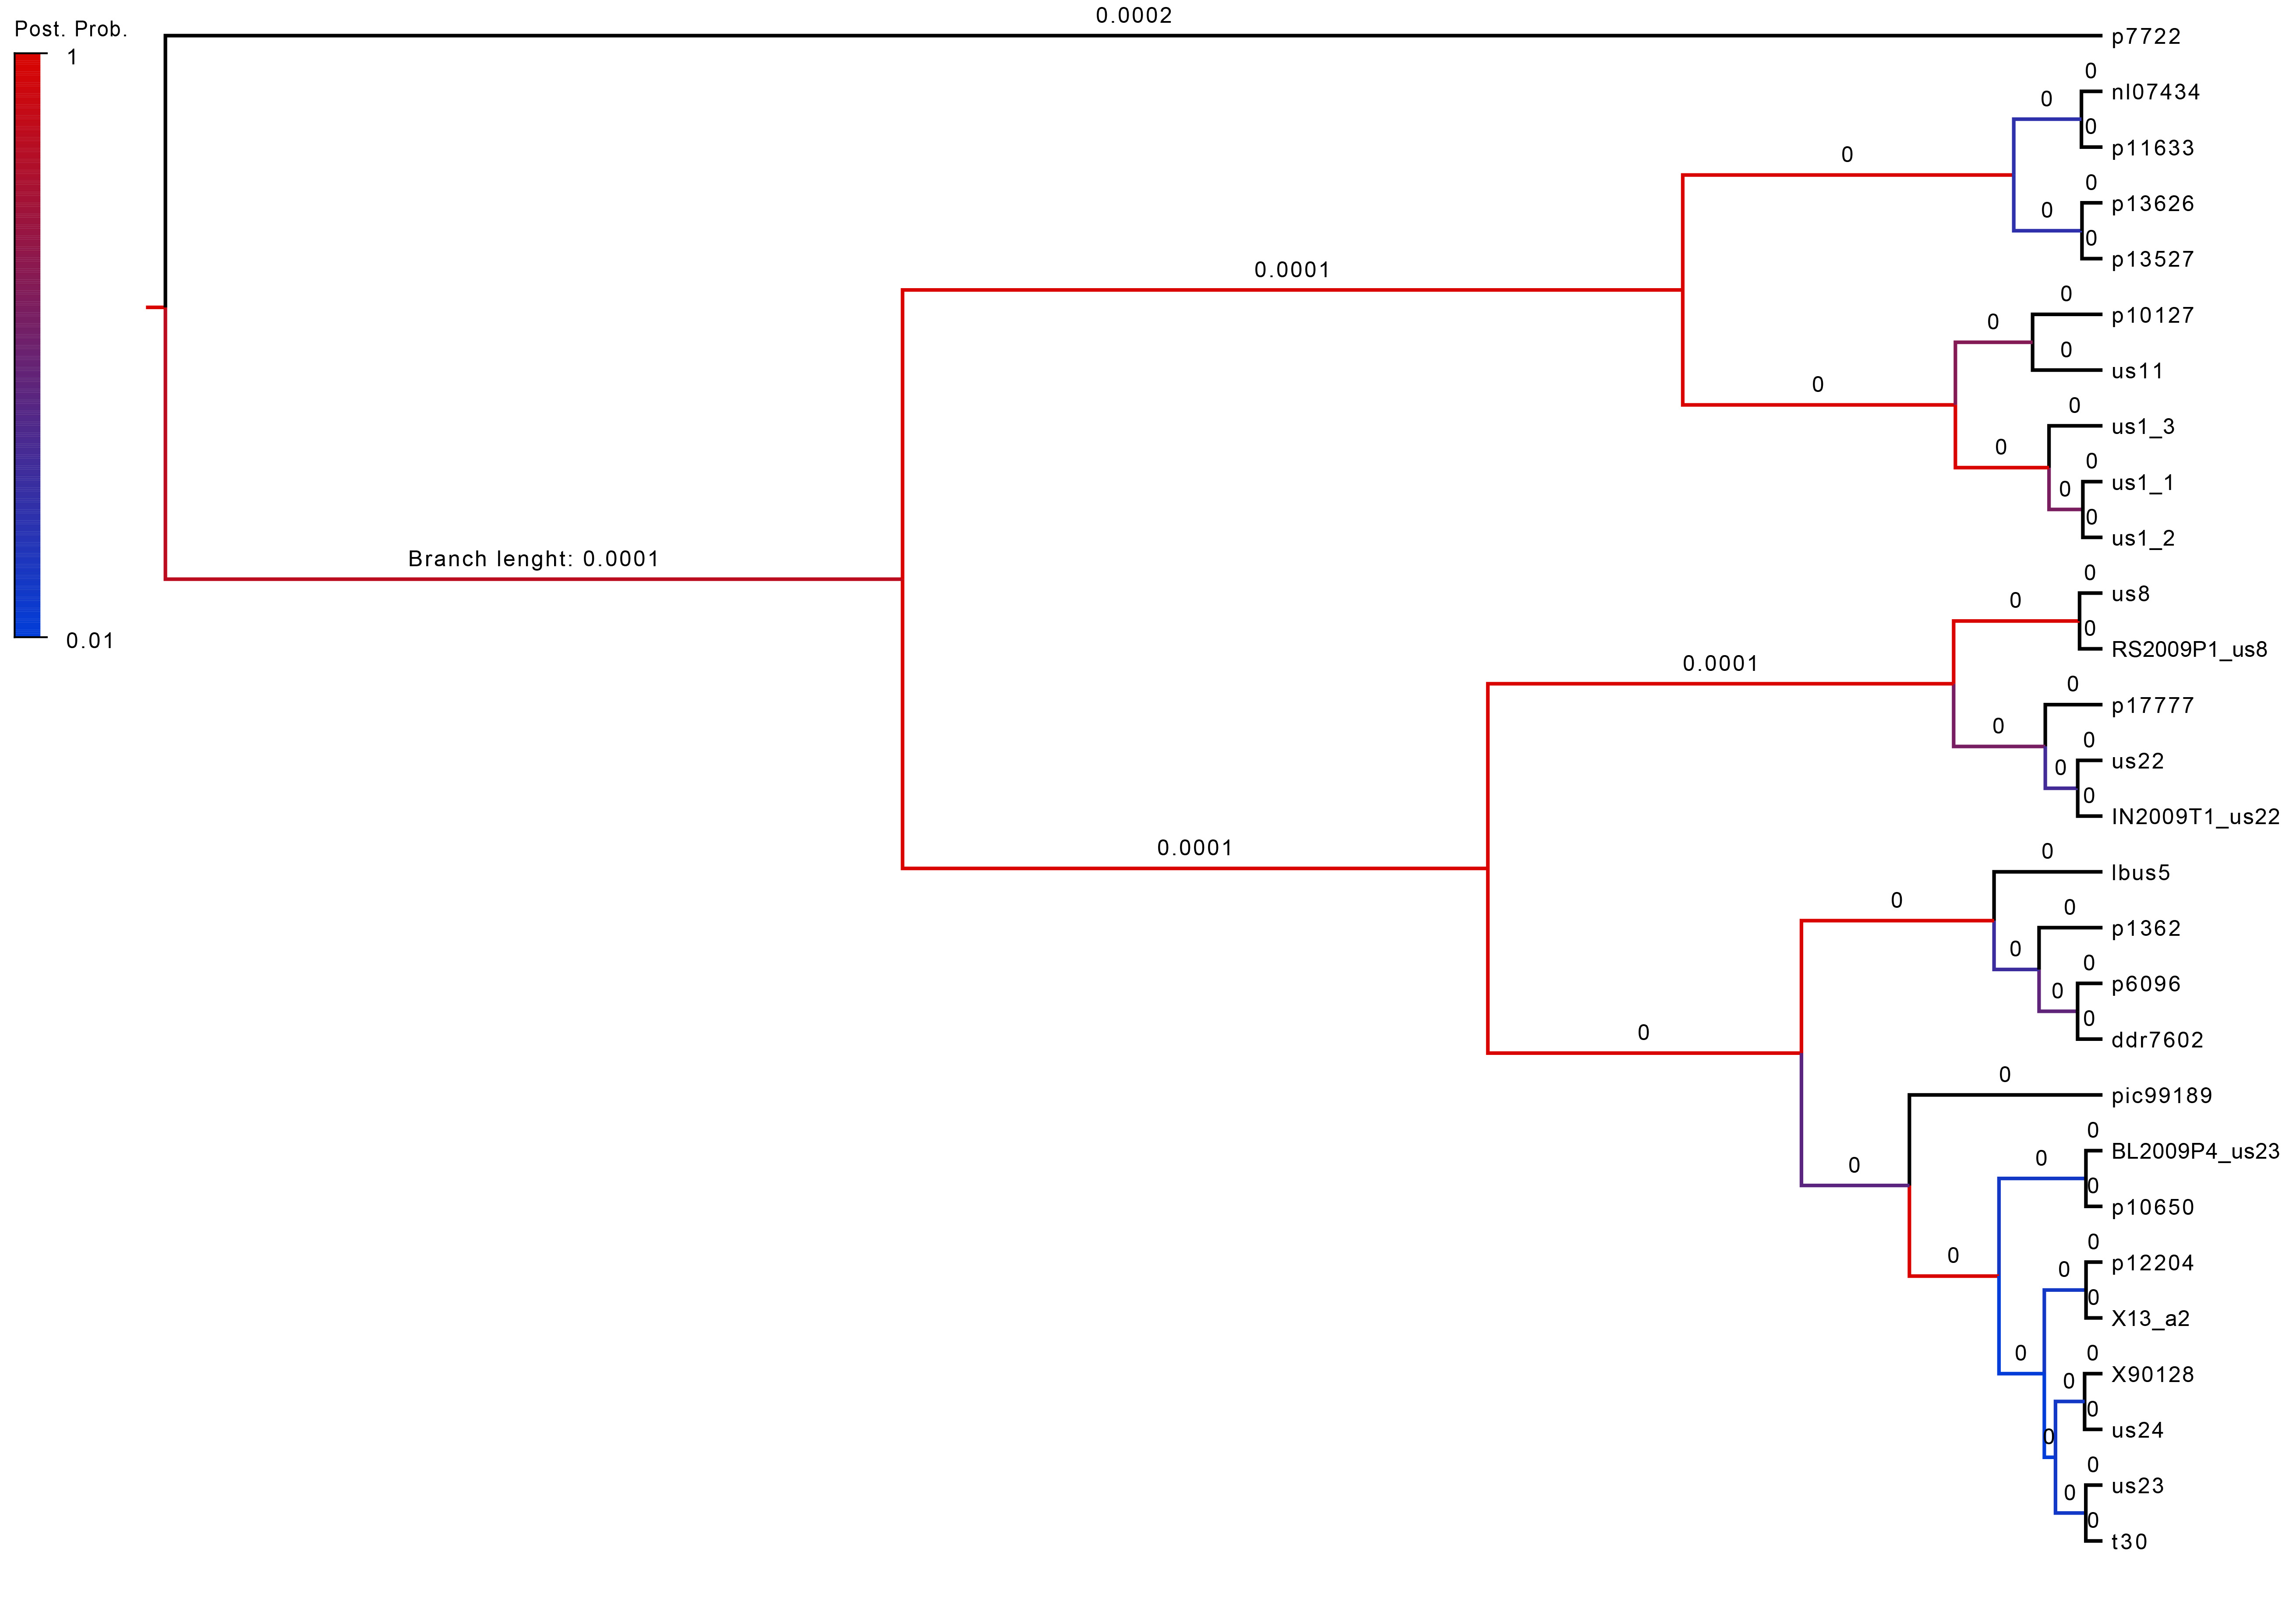
\includegraphics[scale=0.3]{Beast_branchlenghts.jpg}
\caption[BEAST Coalescent tree]{Bayesian coalescent tree of the whole mtDNA genome of \emph{P.infestans} using \texttt{BEAST 1.8.0}. Values above branches represent branch lengths (tolopogy is cooncordant to the bifurcating model of a coalescent recosntruction). Branches are colored based on their posterior probability values (legend indicates values).}
\label{fig:BEAST}
\end{figure}

\subsection{Mapping the SNP's in the BEAST tree}

To map the variants found in the mtDNA genome to the coalescent tree, we used \texttt{Mesquite}. We did a removal of invariable regions and ancestral state reconstruction for all 31 SNPs using a parsimony reconstruction state (Figure \ref{fig:SNP_Trace}).
\newpage
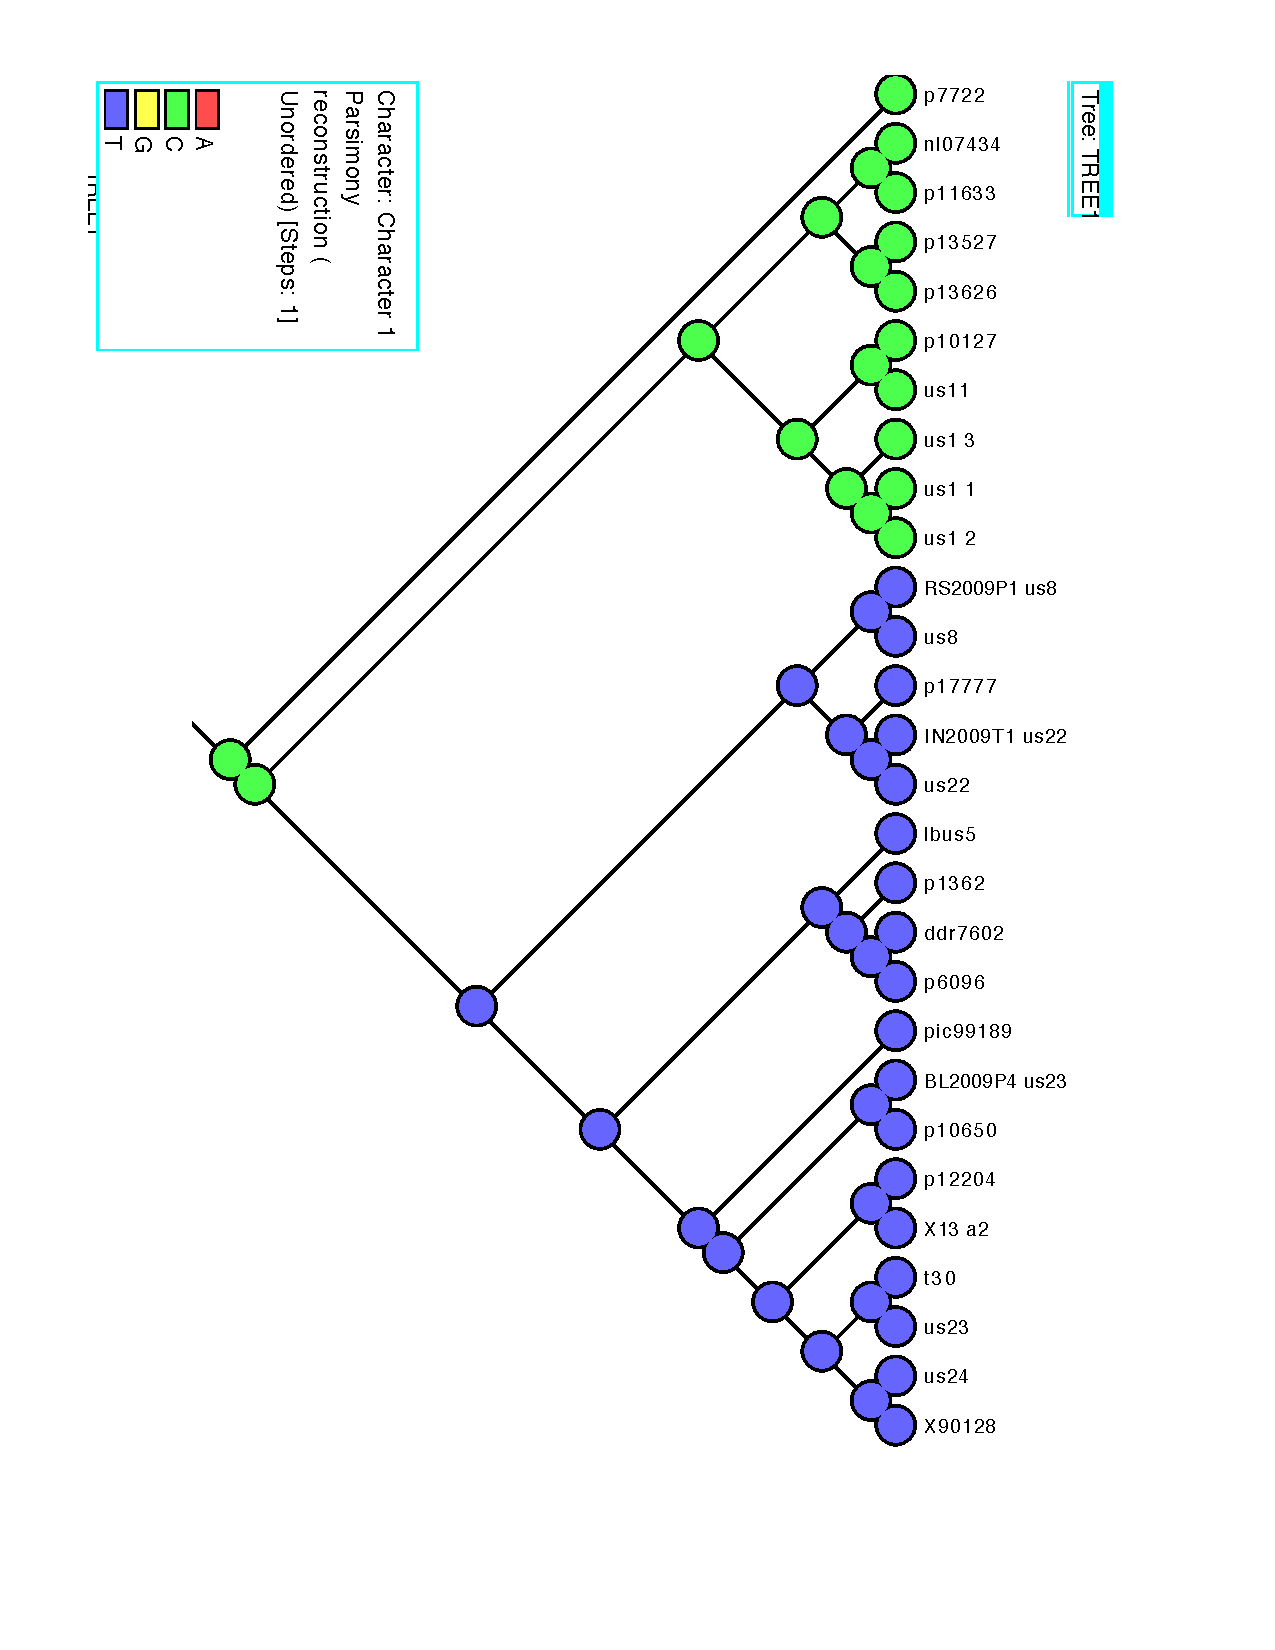
\includepdf[pages={-}, nup=2x2]{All_traces.pdf}


\vspace{24pt}

%% ---------- ---------- ---------- Section ---------- ---------- ---------- %%

\section{Session Information}

\begin{knitrout}
\definecolor{shadecolor}{rgb}{0.969, 0.969, 0.969}\color{fgcolor}\begin{kframe}
\begin{alltt}
\hlkwd{sessionInfo}\hlstd{()}
\end{alltt}
\begin{verbatim}
## R version 3.0.2 (2013-09-25)
## Platform: x86_64-pc-linux-gnu (64-bit)
## 
## locale:
##  [1] LC_CTYPE=en_US.UTF-8       LC_NUMERIC=C              
##  [3] LC_TIME=en_US.UTF-8        LC_COLLATE=en_US.UTF-8    
##  [5] LC_MONETARY=en_US.UTF-8    LC_MESSAGES=en_US.UTF-8   
##  [7] LC_PAPER=en_US.UTF-8       LC_NAME=C                 
##  [9] LC_ADDRESS=C               LC_TELEPHONE=C            
## [11] LC_MEASUREMENT=en_US.UTF-8 LC_IDENTIFICATION=C       
## 
## attached base packages:
## [1] stats     graphics  grDevices utils     datasets  methods   base     
## 
## other attached packages:
## [1] xtable_1.7-1 vcfR_0.1     knitr_1.5   
## 
## loaded via a namespace (and not attached):
## [1] ape_3.0-11      evaluate_0.5.1  formatR_0.10    grid_3.0.2     
## [5] lattice_0.20-24 nlme_3.1-111    stringr_0.6.2   tools_3.0.2
\end{verbatim}
\end{kframe}
\end{knitrout}


%% ---------- ---------- ---------- Section ---------- ---------- ---------- %%

\bibliographystyle{plain}
\bibliography{lineages.bib}

%% ---------- ---------- ---------- Section ---------- ---------- ---------- %%

\end{document}
